%& /home/natalia/.config/TikzEdtWForms/TikzEdtWForms/0.2.1.0/temp_header
\begin{document}
\usetikzlibrary{arrows}
\usetikzlibrary{decorations.pathreplacing}

\begin{tikzpicture}
\shadedraw [draw=none, bottom color={rgb,255:red,4;green,37;blue,35},top color={rgb,255:red,74;green,158;blue,175}] (-13.2,-1.4) rectangle (4,-6.3);
\shadedraw [draw=none, bottom color={rgb,255:red,74;green,158;blue,175},top color={rgb,255:red,121;green,200;blue,230}] (-13.2,-1.4) rectangle (4.05,1.51);
\node(myfirstpic) at (-4.6,3.65) {
\includegraphics[height=.15\textheight,width=0.8\textwidth]{nubes2.png}};


\node (v3) at (-13.25,1.5) {};
\node (v7) at (-7.1,1.5) {};
\node (v8) at (-1.2,1.5) {};
\node (v4) at (4,1.5) {};


\node[] at (2.05,3.8) {\LARGE{\bf Dust}};

\node at (-10.8,3) {\LARGE{\bf CO$_2$}};


\node at (2.1,1.3) {\LARGE{\bf Fe}};
%\draw [double distance=2pt] (v3) edge (v4);
\node (v5) at (-13.2,-1.4) {};
\node (v6) at (4,-1.4) {};
\draw [very thick,dotted] (v5) edge (v6);

\draw [very thick,fill={rgb,255:red,121;green,200;blue,230}] plot[smooth, tension=.7] coordinates {(v3) (-10.2,2.2) (v7) (-4,2) (v8) (1.6,2) (v4)};

\node (v1) at (2.1,3.5) {};
\node (v2) at (2.1,1.8) {};

\draw [ultra thick,-triangle 60,red] (v1) edge (v2);


\draw [very thick,-triangle 60](-6,-2.1) arc (-118.0434:-101.5319:3.15);

\draw[white] [thick,decorate, decoration={brace, amplitude=5pt}](v4) -- (v6);
\node[text width=3.5cm,align=center,rotate=-90] at (4.9,0.1) {\bf Euphotic zone \ "Production zone"};

\draw  (2.9,-1.65) ellipse (0.07 and 0.07);
\draw[fill=gray]  (2.9,-1.65) ellipse (0.03 and 0.03);

\draw  (1.7,-1.4) ellipse (0.07 and 0.07);
\draw[fill=gray]  (1.7,-1.4) ellipse (0.03 and 0.03);

\draw  (3.2,-1.8) ellipse (0.07 and 0.07);
\draw[fill=gray]  (3.2,-1.8) ellipse (0.03 and 0.03);

\draw  (2.9,-1.2) ellipse (0.07 and 0.07);
\draw[fill=gray]  (2.9,-1.2) ellipse (0.03 and 0.03);

\draw  (2.5,0.1) ellipse (0.07 and 0.07);
\draw[fill=gray]  (2.5,0.1) ellipse (0.03 and 0.03);

\draw  (2.15,-3.5) ellipse (0.07 and 0.07);
\draw[fill=gray]  (2.15,-3.5) ellipse (0.03 and 0.03);

\draw  (2.3,-1.2) ellipse (0.07 and 0.07);
\draw[fill=gray]  (2.3,-1.2) ellipse (0.03 and 0.03);

\draw  (2.6,-1.5) ellipse (0.07 and 0.07);
\draw[fill=gray]  (2.6,-1.5) ellipse (0.03 and 0.03);

\draw  (3.1,-0.35) ellipse (0.07 and 0.07);
\draw[fill=gray]  (3.1,-0.35) ellipse (0.03 and 0.03);

\draw  (1.7,-0.8) ellipse (0.07 and 0.07);
\draw[fill=gray]  (1.7,-0.8) ellipse (0.03 and 0.03);

\draw  (2.8,-0.65) ellipse (0.07 and 0.07);
\draw[fill=gray]  (2.8,-0.65) ellipse (0.03 and 0.03);

\draw  (2.35,-0.8) ellipse (0.07 and 0.07);
\draw[fill=gray]  (2.35,-0.8) ellipse (0.03 and 0.03);

\draw  (3.1,-0.8) ellipse (0.07 and 0.07);
\draw[fill=gray]  (3.1,-0.8) ellipse (0.03 and 0.03);


\draw  (3.15,-3.5) ellipse (0.07 and 0.07);
\draw[fill=gray]  (3.15,-3.5) ellipse (0.03 and 0.03);

\draw  (2.7,-3.8) ellipse (0.07 and 0.07);
\draw[fill=gray]  (2.7,-3.8) ellipse (0.03 and 0.03);


%%%

\draw  (2.6,1.05) ellipse (0.07 and 0.07);
\draw[fill=gray]  (2.6,1.05) ellipse (0.03 and 0.03);

\draw  (2.3,-4.1) ellipse (0.07 and 0.07);
\draw[fill=gray]  (2.3,-4.1) ellipse (0.03 and 0.03);

\draw  (2.4,0.7) ellipse (0.07 and 0.07);
\draw[fill=gray]  (2.4,0.7) ellipse (0.03 and 0.03);

\draw  (3.6,-4.4) ellipse (0.07 and 0.07);
\draw[fill=gray]  (3.6,-4.4) ellipse (0.03 and 0.03);

\draw  (3,-4.7) ellipse (0.07 and 0.07);
\draw[fill=gray]  (3,-4.7) ellipse (0.03 and 0.03);

\draw  (2.55,-5.3) ellipse (0.07 and 0.07);
\draw[fill=gray]  (2.6,-5.3) ellipse (0.03 and 0.03);

\draw  (3.35,-5.6) ellipse (0.07 and 0.07);
\draw[fill=gray]  (3.35,-5.6) ellipse (0.03 and 0.03);
%
\draw  (2.65,-1.85) ellipse (0.07 and 0.07);
\draw[fill=gray]  (2.65,-1.85) ellipse (0.03 and 0.03);

\draw  (2.2,-2) ellipse (0.07 and 0.07);
\draw[fill=gray]  (2.2,-2) ellipse (0.03 and 0.03);

\draw  (2.95,-2) ellipse (0.07 and 0.07);
\draw[fill=gray]  (2.95,-2) ellipse (0.03 and 0.03);

\draw  (3.25,-2.15) ellipse (0.07 and 0.07);
\draw[fill=gray]  (3.25,-2.15) ellipse (0.03 and 0.03);

\draw  (2.65,-2.45) ellipse (0.07 and 0.07);
\draw[fill=gray]  (2.65,-2.45) ellipse (0.03 and 0.03);

\draw  (2.2,-2.75) ellipse (0.07 and 0.07);
\draw[fill=gray]  (2.2,-2.75) ellipse (0.03 and 0.03);

\draw  (3,-2.75) ellipse (0.07 and 0.07);
\draw[fill=gray]  (3,-2.75) ellipse (0.03 and 0.03);






\draw [thick,red,-triangle 60](-11,2.8) -- (-11,1);
\draw [red,thick,-triangle 60](-10.5,1) -- (-10.5,2.8);

\draw[gray,thick,loosely dashed] [-open triangle 45](3,1.3) -- (3,-6);

\node[text width=3.7cm,align=center,rotate=-90] at (4.9,-3.7) {\bf Ocean interior \ "Consumption zone"};
\draw [decorate, decoration={brace, amplitude=9pt}](4,-1.4) -- (4,-6.3);
\draw [decorate, decoration={brace, amplitude=10pt}](4,1.7) -- (4,-1.4);
\draw [decorate, decoration={brace, amplitude=5pt}](1.9,1.1) node (v9) {};
\draw[thick,-triangle 60] (1.6,1.2) -- (0.2,1.2);
\draw[thick,-triangle 60] (v9) -- (0.7,0.1);
\draw[thick,-triangle 60] (-5.9,-5.1) -- (-5.9,-5.9);
\node at (-0.5,1.2) {\bf Fe$\bf ^{3+}_{Ligand}$};
\node at (0.2,0.1) {\bf Fe$\bf ^{3+}_{free}$};
\node[left] at (-3.1,-5.8) {\bf Particulate Fe};
\draw[white,ultra thick,loosely dashed]  (-1.2,1.5) rectangle (0.7,-0.2);
\draw[thick] [decorate, decoration={brace, amplitude=9pt},rotate=0](-1.2,0) -- (-1.2,1.5);
\node at (-2.1,0.8) {\bf TDFe};
\node at (-10.7,0.8) {\bf DIC};
%\node(myfirstpic) at (-6.5,1) {\includegraphics[height=.025\textheight]{fito2.png}};
\node[black!30!gray,rotate=270] at (3.5,-2.5) {\bf Sink};
\draw[thick,-triangle 60] (-2.7,0.8) -- (-5,0.8);
\draw[thick,-triangle 60] (-10.1,0.8) -- (-8,0.8);
\draw[red,thick,-triangle 60] (-6,1.5) -- (-5.5,2.5);
\node at (-5.5,2.7) {\bf O$_2$};
\node [
    bottom color=darkgray,
    top color=lightgray,
    opacity=0.5,
    single arrow,
    minimum height=2cm,rotate=-90,
    single arrow head indent=0cm,
     inner sep=8pt,
] at (-6.5,-0.5) {};
%\draw  (-6.5,-2) ellipse (0.07 and 0.07);
\draw[fill=black!30!brown]  (-6.5,-2.2) ellipse (0.05 and 0.05); 
\draw[fill=black!30!brown]  (-6.6,-1.8) ellipse (0.05 and 0.05);
\draw[fill=black!30!brown]  (-6.5,-1.2) node (v10) {} ellipse (0.05 and 0.05); 
\draw[fill=black!30!brown]  (-6.6,-0.7) ellipse (0.05 and 0.05);
\draw[fill=black!30!brown]  (-6.4,0.2) ellipse (0.05 and 0.05); 
\draw[fill=black!30!brown]  (-6.5,-0.2) ellipse (0.05 and 0.05);
\draw[fill=black!30!brown]  (-6.6,0.1) ellipse (0.05 and 0.05); 
\draw[fill=black!30!brown]  (-6.5,-0.55) ellipse (0.05 and 0.05);
\draw[fill=black!30!brown]  (-6.4,-2.1) ellipse (0.05 and 0.05); 
\draw[fill=black!30!brown]  (-6.3,-1.7) ellipse (0.05 and 0.05);
\draw[fill=black!30!brown]  (-6.4,-3.1) ellipse (0.05 and 0.05); 
\draw[fill=black!30!brown]  (-6.3,-3) ellipse (0.05 and 0.05);
\draw[fill=black!30!brown]  (-6.5,-4.2) ellipse (0.05 and 0.05);
\draw[fill=black!30!brown]  (-6.6,-4) ellipse (0.05 and 0.05);

\draw[fill=black!30!brown]  (-6.5,-5) ellipse (0.05 and 0.05);
\draw[fill=black!30!brown]  (-6.3,-5.5) ellipse (0.05 and 0.05);
\draw[fill=black!30!brown]  (-6,-5.2) ellipse (0.05 and 0.05);
\draw[fill=black!30!brown]  (-6.2,-4.7) ellipse (0.05 and 0.05);
\draw[fill=black!30!brown]  (-6.1,-3.7) ellipse (0.05 and 0.05);
\draw[fill=black!30!brown]  (-6.4,-3.5) ellipse (0.05 and 0.05);
\node[black!60!green ] at (-6.5,0.6) {\bf Phytoplankton};
\node at (-7.5,-0.65) {\bf POM};
\node at (-5.5,-0.65) {\bf DOM};
\draw[thick,-triangle 60] (-6.1,0.5) node (v11) {} -- (-4.7,0);
\node at (-4.5,-0.1) {\bf O$_2$};
\draw[fill=brown]  (-4.5,-2.49) ellipse (0.05 and 0.12); 
\draw[fill=brown]  (-4,-2.69) ellipse (0.12 and 0.05);
\draw[fill=brown]  (-3.5,-2.09) ellipse (0.05 and 0.12); 
\draw[fill=brown]  (-4.3,-2.39) ellipse (0.12 and 0.05);
\draw[fill=brown]  (-3.3,-1.94) ellipse (0.05 and 0.12); 
\draw[fill=brown]  (-4.8,-2.89) ellipse (0.12 and 0.05);
\draw[fill=brown]  (-4.2,-1.88) ellipse (0.05 and 0.12); 
\draw[fill=brown]  (-3.5,-3.09) ellipse (0.12 and 0.05);
\draw[fill=brown]  (-4.5,-3.29) ellipse (0.05 and 0.12); 
\draw[fill=brown]  (-3,-2.29) ellipse (0.12 and 0.05);
%
\draw[fill=black!30!brown]  (-4.5,-2.29) ellipse (0.05 and 0.05);
\draw[fill=black!30!brown]  (-5,-1.99) ellipse (0.05 and 0.05);
\draw[fill=black!30!brown]  (-4.1,-2.39) ellipse (0.05 and 0.05);
\draw[fill=black!30!brown]  (-4.2,-2.79) ellipse (0.05 and 0.05);
%\draw[fill=black!30!brown]  (-5,-2) ellipse (0.05 and 0.05);
\draw[fill=black!30!brown]  (-4.8,-2.03) ellipse (0.03 and 0.03);
\draw[fill=black!30!brown]  (-4.1,-2.54) ellipse (0.03 and 0.03);
\draw[fill=black!30!brown]  (-3.5,-2.79) ellipse (0.03 and 0.03);
\draw[fill=black!30!brown]  (-4,-2) ellipse (0.03 and 0.03);
\draw[fill=black!30!brown]  (-3.8,-2.54) ellipse (0.03 and 0.03);
\draw[fill=black!30!brown]  (-3.3,-2.79) ellipse (0.03 and 0.03);
\draw[fill=black!30!brown]  (-2.5,-2.03) ellipse (0.03 and 0.03);
\draw[fill=black!30!brown]  (-3,-2.52) ellipse (0.03 and 0.03);
\draw[fill=black!30!brown]  (-3.5,-2.84) ellipse (0.03 and 0.03);
\node[black!70!brown] at (-4.3,-3.09) {\bf Bacteria};
\draw[very thick,-triangle 60]  plot[smooth, tension=.7] coordinates {(-6,-3.3) (-5.7,-3) (-5.2,-2.8)};
\draw[gray,very thick,loosely dashed]  (-4,-2.5) ellipse (1.8 and 1.3);
\node[black!30!gray] at (-4.1,-1.6) {\bf Remineralization};
\draw[thick,-triangle 60] (-2.1,-2.9) -- (-1.2,-3.3);
\node at (-1,-3.6) {\bf C$\bf _{reg}$};
%\draw[loosely dashed,gray,thick,-triangle 60] (-0.3,-3.5) -- (1.5,-3.5);
%\node[gray] at (0.4,-3.2) {\bf Scavenging};
\draw[thick,-triangle 60] (-8.6,-0.2) -- (-7.3,0.4);
\node at (-9.1,-0.3) {\bf PO$\bf _{4}^{3-}$};
\draw[thick,-triangle 60] (-0.9,-1.9) -- (-2.1,-2.2);
%\node[text width=2cm,align=center] at (-0.2,-1.9) {R$_{Red}$ \\ (N:P:O$_{2}$:H)};
\node[text width=2cm,align=center] at (-0.6,-1.9) {\bf O$\bf _{2}$};
%\node[gray] at (-6.5,-1) {\bf Export};
\node[gray,rotate=90] at (2.5,-4.6) {\bf SinK};
\draw[gray,thick,-triangle 60,loosely dashed] (-7.1,-3.2) -- (-7.1,-6);
\draw (v10) -- cycle;
\node[gray,rotate=90] at (-7.5,-4.6) {\bf Sink};
\node[white] at (-6.7,-1) {P};
\node[white] at (-6.2,-1) {Fe};
\draw[thick,-triangle 60] (-3.7,-3.6) -- (-3.7,-4.4);
\node at (-3.6,-4.6) {\bf Fe$_{reg}$};
% \draw[thick,-triangle 60] (-3.8,-4.6) -- (-4.1,-4.9);
% \node at (-4.3,-5.1) {Fe$^{3+}_{free}$};
% \draw[thick,-triangle 60] (-3.6,-4.6) -- (-3.3,-4.9);
\draw[loosely dashed,gray,thick,triangle 60-triangle 60] (-3.2,-4.5) -- (-1,-4.5);
\node at (-0.7,-4.6) {\bf L$\bf_{free}$};
\draw[gray,loosely dashed, thick,-triangle 60] (-4.3,-4.5) -- (-5.2,-4.5);
\node[gray] at (-4.8,-4.9) {\bf Scavenging};
\node[gray] at (-2,-4.2) {\bf Complexation};
\draw[thick,-triangle 60] (v11) -- (-3,0.1);
\node at (-2.5,0.1) {\bf L$\bf _{free}$};
\draw[white,dotted,thick,stealth-stealth]  plot[smooth, tension=.7] coordinates {(0.5,-1) (0.1,-1.2) (0.6,-1.5) (0.3,-1.8)};
\draw[white,dotted,thick,stealth-stealth]  plot[smooth, tension=.7] coordinates {(0.9,-1) (0.5,-1.2) (1,-1.5) (0.7,-1.8)};
\draw[white,dotted,thick,stealth-stealth]  plot[smooth, tension=.7] coordinates {(-10,-1) (-9.6,-1.2) (-10.1,-1.5) (-9.8,-1.8)};
\draw[white,dotted,thick,stealth-stealth]  plot[smooth, tension=.7] coordinates {(-10.4,-1) (-10,-1.2) (-10.5,-1.5) (-10.2,-1.8)};
\draw[white,dotted,thick,stealth-stealth]  plot[smooth, tension=.7] coordinates {(-2.9,-1) (-2.4,-1.2) (-1.9,-1)};
\draw[white,dotted,thick,stealth-stealth]  plot[smooth, tension=.7] coordinates {(-1.9,-0.7) (-2.4,-0.5) (-2.9,-0.7)};
\draw[white,dotted,thick,stealth-stealth]  plot[smooth, tension=.7] coordinates {(-13,-1) (-12.5,-1.2) (-12,-1)};
\draw[white,dotted,thick,stealth-stealth]  plot[smooth, tension=.7] coordinates {(-12,-0.7) (-12.5,-0.5) (-13,-0.7)};
\draw[loosely dashed,gray,thick,triangle 60-triangle 60] (-2,0.1) -- (-0.5,0.1);
\node[black!20!gray] at (-1.3,-0.3) {\bf Complexation};
\draw[loosely dashed,gray,thick,-triangle 60] (0.7,0.1) -- (2.2,0.1);
\node[black!20!gray] at (1.9,-0.3) {\bf Scavenging};
\draw[thick,-triangle 60] (2.6,1.2) -- (3.3,1.2);
\node[rotate=-90] at (3.5,0.3) {\bf Particulate Fe};
\draw[thick,-triangle 60] (-2.1,-2.6) -- (-1.2,-2.6);
\node at (-0.8,-2.6) {\bf P$\bf _{reg}$};
\node at (-6.5,1.1) {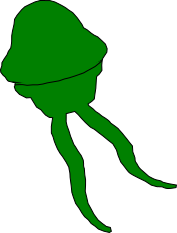
\includegraphics[height=.02\textheight]{fito_1.png}};
\node at (-6.1,1) {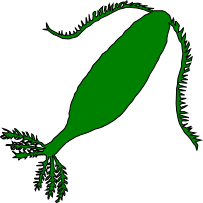
\includegraphics[height=.018\textheight]{fito_2.png}};
\node at (-6.9,1) {
\includegraphics[height=.018\textheight]{fito_3.png}};
\node at (-7.6,1.2) {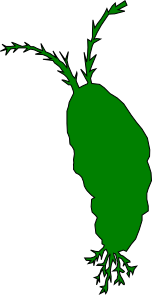
\includegraphics[height=.023\textheight]{fito_4.png}};
\node at (-5.6,1.4) {
\includegraphics[height=.018\textheight]{fito_5.png}};
\node at (-8,1.2) {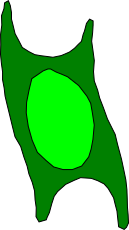
\includegraphics[height=.02\textheight]{fito_6.png}};
\node at (-7.2,1.1) {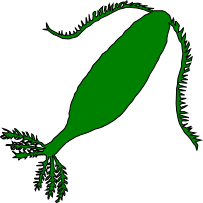
\includegraphics[height=.018\textheight]{fito_2.png}};
\node at (-5.53,0.63) {
\includegraphics[height=.01\textheight]{fito_3.png}};
\node at (-5.2,1.1) {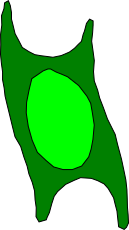
\includegraphics[height=.02\textheight]{fito_6.png}};
\node at (-6,-2.5) {\bf POM};

\usetikzlibrary{calc}
\pgftransformreset
\node[inner sep=0pt,outer sep=0pt,minimum size=0pt,line width=0pt,text width=0pt,text height=0pt] at (current bounding box) {};
%add border to avoid cropping by pdflibnet
\foreach \border in {0.1}
  \useasboundingbox (current bounding box.south west)+(-\border,-\border) rectangle (current bounding box.north east)+(\border,\border);
\newwrite\metadatafile
\immediate\openout\metadatafile=\jobname_BB.txt
\path
  let
    \p1=(current bounding box.south west),
    \p2=(current bounding box.north east)
  in
  node[inner sep=0pt,outer sep=0pt,minimum size=0pt,line width=0pt,text width=0pt,text height=0pt,draw=white] at (current bounding box) {
\immediate\write\metadatafile{\p1,\p2}
};
\immediate\closeout\metadatafile
\end{tikzpicture}

\end{document}
